

\chapter{Bewertungskriterien}
\label{ch:Bewertungskriterien}
In diesem Kapitel werden die für eine Eignung bzw. Uneignung benötigten Kriterien vorgestellt.\\
Die Bewertungskriterien sind notwendig, um eine Modellierugnssprache zu bewerten. Da die Modellierungssprachen unterschiedliche Eigenschaften, Spzifikationen und Benutzungszweck haben, lässt sich eine liste von verchiedene Kategorien der Kirtirien  schwierig zu bestimmen.\\
Die Eignungskriterien treffen auf verschiedenste Arten von Modellierungssprachen zu. In diesem Abschnitt werden diese Kriterien in drei Hauptkategorie aufgeteilt: Formale- , Anwenderbezogene- und Anwendungsbezogene -Kriterien. Danach werden diese im Verlauf in weiteren Kategorien aufgeteilt.
Die Bewertungen sind oft von dem Bewerter und dem Benutzer abhängig, z.b. kann jemand eine Modellierungssprache sehr einfach finden, wenn jemand anders sie schwierig findet, deswegen gibt es manchmal kein bestimmte Bewertungsverfahren und sichere Entscheidung, ob das Merkmal erfüllt ist.\\

Die Kriterien sind in drei Kategorien eingeteilt, auf welche im Folgenden eingegangen wird:

\begin{itemize}
	\item Formale Kriterien
	\item Anwenderbezogene Kriterien
	\item Anwendungsbezogene Kriterien
\end{itemize}


\section{Formale Kriterien}  
Diese Kriterien dienen der maschinellen Prüfung von Modellen sowie der Berechnung von Modelleigenschaften. Werden die Anforderungen von der Modellierungssprache erfüllt, kann ein mit ihr geschaffenes Prozessmodell z. B. auf syntaktische Korrektheit überprüft werden. Die formalen Kriterien spielen eine besondere Rolle, wenn für die Modellierung Softwarewerkzeuge eingesetzt werden.\cite{MT007} \\
Die formalen Kriterien werden in die fünf Einzelkriterien Korrektheit, Vollständigkeit, Einheitlichkeit, Redundanzfreiheit und Struktureierbarkeit unterteilt.
\subsection{Korrektheit}
Eine Modellierungssprache genügt dem Kriterium der Korrektheit, wenn sie unzulässige Modelle eindeutig identifiziert und gleichzeitig erlaubt, die Menge aller zulässigen Modelle zu generieren. Zu unterscheiden ist dabei die syntaktische Korrektheit sowie die semantische Korrektheit der Modelle. Die semi-formalen Prozessmodellierungssprachen, welche für die Prozessdokumentation in Frage kommen, besitzen in der Regel keine eindeutig festgelegte Semantik, sodass hier vor allem die Möglichkeit der automatischen Überprüfung einer korrekten Syntax des Modells im Vordergrund steht. Das Kriterium der Korrektheit steht in enger Verbindung zum Grundsatz der Richtigkeit der Grundsätze ordnungsgemäßer Modellierung.\cite{MT007}
\subsection{Vollständigkeit}
Unter Vollständigkeit wird in diesem Zusammenhang die Vollständigkeit der Sprachbeschreibung verstanden. Alle Konstrukte sowie die Bedingungen ihrer Verwendung, die von der Modellierungssprache bereitgestellt werden, müssen eindeutig definiert und beschrieben sein.\cite{MT007}
\subsection{Einheitlichkeit}
Das Kriterium der Einheitlichkeit ist angelehnt an den Grundsatz der Klarheit der Grundsätze ordnungsmäßiger Modellierung. Einheitlichkeit bedeutet in diesem Kontext, dass alle Konstrukte der Sprache verständlich dargestellt und beschrieben werden. Ähnliche Konstrukte sollten somit auch in ähnlicher Weise spezifiziert werden.
\subsection{Redundanzfreiheit}
Die Redundanzfreiheit setzt voraus, dass die Sprache keine Mehrfachdefinition von Konstrukten vornimmt, die denselben Sachverhalt beschreiben. Ein und derselbe Sachverhalt sollte also nicht mit mehreren verschiedenen Elementen bzw. Symbolen der Modellierungssprache belegt sein. Auch dieses Kriterium fördert den Grundsatz der Klarheit. Indem gleiche realweltliche Sachverhalte in der Modellierungssprache durch gleiche Konstrukte ausgedrückt werden, wird zudem der Grundsatz der Vergleichbarkeit gefördert.
\subsection{Strukturierbarkeit}
Da Informationsmodelle eine hohe Komplexität aufweisen können, sollte die Sprache Konstrukte bereitstellen, welche die Strukturierung der modellierten Informationen unterstützt. Die Modellierungssprache muss also Zerlegungen in Prozesskomponenten oder Teilprozesse darstellen können. Die Schnittstellen zwischen den Komponenten müssen übersichtlich dargestellt werden. Verallgemeinerungen (Generalisierung) und Detaillierungen (Spezialisierung) müssen schlüssig nachvollziehbar sein. Die Strukturierung in Teilmodelle ermöglicht gleichzeitig die Wiederverwendbarkeit der Strukturen in anderen Modellen. So können etwa modellierte Teilprozesse in anderen Prozessen wieder aufgegriffen werden und müssen nicht mehrfach modelliert werden. Zusätzlich wird dadurch die Wartbarkeit der Modelle verbessert, da Änderungen in einem Modellteil, die Konsistenz der übrigen Modellteile nicht beeinflussen. Das Kriterium der Strukturierbarkeit unterstützt den Grundsatz des systematischen Aufbaus der Grundsätze ordnungsgemäßer Modellierung
\section{Anwenderbezogene Kriterien}
\label{sc:AnwenderbezogeneKriterien}
Die anwenderbezogenen Kriterien beschreiben das Verhältnis zwischen dem Anwender und der verwendeten Modellierungssprache. Der Anwender kann zum einen der Modellierer und zum anderen der Betrachter eines Modells sein. Die anwenderbezogenen Kriterien besitzen eine besondere Bedeutung, um Nutzern von Modellen das Verständnis zu erleichtern bzw. zu ermöglichen. Für den betrachteten Anwendungsfall der Prozessdokumentation, zur Nutzung als allgemeine Arbeitsgrundlage für die Mitarbeiter einer Organisation, spielen sie daher eine sehr große Rolle. Die Modellierungssprache ermöglicht das Erstellen von Modellen, um Ideen und Gedanken zwischen den Beteiligten auszutauschen. Sie sind somit in erster Linie für den menschlichen Anwender als Kommunikationsmittel zu verstehen.\cite{MT007}   
\subsection{Einfachheit und Erlernbarkeit}
Das Kriterium der Einfachheit geht von folgendem Prinzip aus: Je einfacher eine Sprache ist, desto weniger Fehler sind bei der Modellierung mit ihr zu erwarten. Die Einfachheit der Modellierungssprache wird bestimmt durch eine geringe Anzahl an Notationselementen und Begriffen, sowie der Verwendung von einfachen Regeln für ihre Anwendung. Der Aspekt betrifft zum einen den Ersteller eines Modells, der bei einfachen Sprachen nur Kenntnis von wenigen Symbolen und Regeln haben muss, um Modelle zu erstellen. Wichtiger sind bei der Prozessdokumentation jedoch die Betrachter der Modelle. Dazu zählen nicht nur Fachexperten, sondern häufig einfache Arbeiter in den Unternehmen. Diese besitzen meist nur sehr eingeschränkte bis gar keine Methodenkenntnisse auf dem Gebiet der Prozessmodellierung. Trotzdem müssen die Modelle verstanden werden, wenn sie als Arbeitsgrundlage Verwendung finden sollen. \\
Eine Sprache, die für die Dokumentation von Prozessen verwendet wird, sollte nicht nur möglichst einfach sein, sondern auch den erforderlichen Schulungsbedarf auf einem akzeptablen Niveau halten. Vom Kriterium der Erlernbarkeit wird also ein möglichst geringer Aufwand zum Erlernen der notwendigen Konstrukte und Regeln der Modellierungssprache gefordert. Dies hängt wiederum stark von der Anzahl der Konstrukte der Sprache ab, sodass die Einfachheit und die Erlernbarkeit sehr stark korrelieren. Deshalb wurden sie in einem gemeinsamen Kriterium zusammengeführt. Das Kriterium der Einfachheit und Erlernbarkeit unterstützt den Grundsatz der Klarheit der GoM. Außerdem wird der Grundsatz der Wirtschaftlichkeit angesprochen, da insbesondere der Schulungsaufwand zum Nachvollziehen der Modellierungssprache und die Ausbildung zur Geschäftsprozessmodellierung in der Organisation einen erheblichen Kostenfaktor darstellen können.
\subsection{Verständlichkeit}
Die Modellierungssprache gilt als verständlich, wenn sie ein dem Nutzer bekanntes Vokabular benutzt, d. h. die definierten Konstrukte sollten im Wesentlichen mit Begriffen korrespondieren, die dem Anwender vertraut sind. Auf den Zweck der Prozessdokumentation übertragen bedeutet dies, dass die Symbole der Notation eher mit betriebswirtschaftlichen und allgemein bekannten Begriffen besetzt sein sollten, als etwa mit Begriffen aus der Softwareentwicklung oder anderen technischen Richtungen. Die Begriffe müssen dem Anwender aus seiner täglichen Arbeit bekannt sein, damit die Bedeutung leicht zu interpretieren ist. Auch die Verständlichkeit einer Modellierungssprache fördert die Qualität des damit abgebildeten Ergebnismodells und unterstützt somit den Grundsatz der Klarheit.

\subsection{Anschaulichkeit}
Während die Verständlichkeit eher auf die Benennung und verständliche Definition der Konstrukte ausgerichtet ist, umfasst das Kriterium der Anschaulichkeit die Forderung nach Struktur, Übersichtlichkeit und Lesbarkeit der Modelle, um den Grundsatz der Klarheit zu fördern. Die grafische Darstellung sollte möglichst intuitive Konzepte einsetzen um die Anschaulichkeit zu erhöhen. Dies kann z. B. die Verwendung von Piktogrammen sein, die real-weltlichen Objekten nachempfunden sind. Die Lesbarkeit sinkt, umso mehr verschiedene Notationselemente verwendet werden. Es wird davon ausgegangen, dass der Mensch durch das direkte Betrachten nur etwa sechs verschiedene Notationselemente unterscheiden kann. Die Struktur beschreibt, wie die Elemente in einem Modell gruppiert werden. So können z. B. Überschneidungen von Kanten die Anschaulichkeit eines Modells erheblich reduzieren.



\section{Anwendungsbezogene Kriterien}
\label{sc:AnwendungsbezogeneKriterien}
Anwendungsbezogene Kriterien beschreiben die Anforderungen einer Modellierungssprache an eine Anwendung innerhalb eines Domänenspezifischen Einsatzes.
Dies hängt von den jeweiligen Aspekten ab, welche durch die Modellierungssprache abgebildet werden soll.
So besitzen verschiedene Modellierungssprachen unter anderem ein unterschiedlich großes Nutzungspotenzial in der jeweiligen Anwendungsdomäne.
Man spricht in diesem Zusammenhang auch von der Mächtigkeit der Sprache.
Dabei ist zu beachten, das Anwendungs- und Anwenderbezogene Kriterien oft konkurrierend sein können,
so kann sich beispielsweise eine leicht erlernbare Sprache sich negativ auf die Mächtigkeit auswirken und umgekehrt.
Anwendungsbezogene Kriterien können in Anforderungen wie der Angemessenheit, der Mächtigkeit, der Operationalisierbarkeit,
und der Überprüfbarkeit beschrieben werden.
Zwar gibt es höchstwahrscheinlich noch eine weit aus größere Anzahl an Kriterien, diese sollen uns aber in dieser Arbeit genügen \cite[95\psq]{JaneFroeming_2009}.
\subsection{Angemessenheit}
\label{ssc:Angemessenheit}
Die Angemessenheit einer Sprache bezieht sich auf die Gesamtheit der Sprache,
als auch auf die einzelnen Konzepte der Sprache und umfasst damit das Abstraktionsniveau, den Detaillierungsgrad und den Formalisierungsgrad einer Sprache \cite[97]{Lobe_2015}.

Die Abstraktionsfähigkeit einer Modellierungssprache beschreibt, worin die Fachterminologie der Domäne sich mit den Konzepten der Modellierungssprache möglichst decken sollte und welche unwesentlichen Details abstrahiert werden. In dem Bereich von Kommunikationsabläufen der Telekommunikation sind diese Begriffe eher technischer Natur und kommen aus einem Informatik-spezifischem Umfeld, welcher Fachsprache auf dem Niveau von Spezialisten voraussetzt. 

Der Detaillierungsgrad beschreibt wie Sachlich angemessen detailliert die Konstrukte eines Anwendungszwecks der Domäne sich darstellen lassen können. Dies beinhaltet die zu Modellierenden Modelle, Daten und zusätzlichen Informationen. Damit ist nicht gemeint, dass ein System in einer hohen Abstraktionsform eine eins zu eins Nachbildung aller technischen Prozesse des Informationssystems ausdrücken soll,
sondern nur für die Zielgruppe angemessene und verständliche Konzepte. Eine formale Beschreibung der Prozesse ist demnach nicht gewünscht, da der Hauptaugenmerk auf dem Anwender liegt.

Die Angemessenheit der Sprache ist abhängig durch den Anwendungszweck.
Da aber der Sachverhalt zumeist unklar definiert ist, ist es nicht immer möglich zu überprüfen ob ein Modell einen Sachverhalt abbildet. Dies ist nicht der Fall, wenn der Sachverhalt exakt definiert ist und eine formale Überprüfung der Angemessenheit vorgenommen werden kann.

Genauso steht sie somit in direktem Zusammenhang mit der Mächtigkeit, einem weiterem Kriterium, welche später in der Arbeit behandelt wird und dem Anwendungszweck einer Sprache. 
So bieten Angemessenheit und Mächtigkeit zusammen die Möglichkeit, die bereitgestellten Konzepte einer Sprache bezogen auf den Anwendungszweck zu untersuchen. Demnach sollen ausreichende Konzepte bereitgestellt werden, ohne jedoch überflüssige Konzepte zu enthalten \cite[35F]{Frank_1997}.

\subsubsection{Konsequenz}
Im Hinblick ob ein Konstrukt der Sprache nun Angemessen ist oder nicht, hängt subjektiv vom jeweiligen Betrachter ab. 
Dies ist insbesondere bei komplizierten Konstrukten Fall. Im Zweifelsfall muss nun entschieden werden, ob es ein notwendiges Sprachkonstrukt darstellt oder ob es nur die Sprachkomplexität erhöht. Dies muss jedoch für jedes einzelne Konstrukt abgewägt werden, da jedes seine eigenen spezifischen Vor- und Nachteile besitzt. Laut Ulrich Frank und Micheal Prasse ist es sogar gar nicht möglich, ein formelles Maß zu Bestimmung von Angemessenheit von Modellierungssprachen zu besitzen, da die Untersuchung eines Konstrukts der Sprache immer nur subjektiv erfolgen kann, man jedoch aber die Bedeutsamkeit des Konstrukts im jeweiligen Anwendungsfalls beurteilen kann \cite[35]{Frank_1997}.

\subsection{Mächtigkeit}
\label{ssc:Nutzungspotenzial}
Die Mächtigkeit ist ein maß des Nutzungspotenzials einer Sprache und gibt Aussage darüber,
in wie weit und wie gut die Konzepte der verwendeten Sprache, die Eigenschaften eines Sachverhalt der Domäne darstellen kann.
Darunter fällt wie Präzise diese Aussagen sind und wie hoch der Detailgrad der darzustellenden Eigenschaft ist \cite[180]{Allweyer_2005}.
Der Sprachumfang korreliert mit der Mächtigkeit der Sprache. Je größer dieser Umfang ist, desto größer ist auch die Mächtigkeit der Sprache.
Da es für den Anwender von großer Bedeutung ist, seine Anwendung mit einem möglichst umfänglichen Detailgrad beschreiben zu können,
muss die Mächtigkeit mindestens alle Aspekte enthalten, die für den gewünschten darzustellenden Sachverhalt notwendig sind.
Eine Mächtigkeit der Sprache, die sich über den Anwendungszweck der Domäne bezieht, kann wie schon erwähnt sich negativ auf andere Kriterien auswirken.
Ferner jedoch, kann man die Mächtigkeit einer formalen Modellierungssprache in der Automatentheorie anhand ihres Grammatik-Typen festlegen.
Eine Modellierungssprache sollte sich auf die Modellierung konzentrieren.
So können zu viele Konzepte zu einer unangemessen mächtigen Sprache führen, was zwangsläufig ihre Komplexität erhöht. Zwischen Mächtigkeit
und Angemessenheit muss daher ein ausgewogenes Verhältnis existieren.

\subsubsection{Konsequenz}
Mächtigkeit und Angemessenheit bedingen einander. Die Mächtigkeit einer Sprache muss daher relativ
zur Anwendungsdomäne betrachtet werden. Geht man grundsätzlich davon aus, dass die hier betrachteten
Modellierungssprachen der konzeptuellen Modellierung dienen, misst sich die Mächtigkeit einerseits
an der Möglichkeit, als wesentlich erkannte Sachverhalte des abzubildenden Realitätsbereichs
natürlich, also ohne aufwendige Rekonstruktionen, beschreiben zu können. Andererseits sollte die
Modellierungssprache auch Möglichkeiten bieten, Informationen darzustellen, die für die Implementierung
benötigt werden.


\subsection{Operationalisierbarkeit}
\label{ssc:Operationalisierbarkeit}
Die Operationalisierbarkeit gibt Aussage darüber, ob und wie gut sich die Modellierungssprache über ihre eigene Verwendung hinaus noch weiter verwenden lässt.
Darunter fällt die Transformation des Modells in andere Sprachen als auch das darstellen von diversen Sachverhalten.
Bei der Transformation ist hierbei zu beachten, dass die verwendeten Konzepte beider Sprachen möglichst gleich sein müssen,
um eine annähernd vollständige Konvertierung zu ermöglichen. Zur Abbildung diverser Sachverhalte enthält eine gute Operationalisierbarkeit die Abbildungsmöglichkeit von Funktionen, Bedingungen, Ressourcen, Objekten und Ereignissen.
Deswegen müssen Konzepte zur Planung und Analyse des domänenspezifischen Einsatzes enthalten sein \cite[95\psq]{JaneFroeming_2009}.

\subsection{Überprüfbarkeit}
Die Überprüfbarkeit eines Modells einer Modellierungssprache bezieht sich auf die Realitätsnähe eines abzubildenden Sachverhalts. Es ist also ein Maß der Abweichung eines Modells, bezogen auf die Realität welches es abbilden soll.
Ein Modell sollte also immer möglichst genau, überprüfbar und nachvollziehbar an der Realität übergreifend für die Betrachter liegen. Dabei muss jedoch berücksichtigt werden, dass objektive Verfahrensweisen für ein Modell nicht vollumfänglich anwendbar sind, da es sich meist um geplante und nicht faktischen Realitäten handelt. Dadurch gegeben obliegt diese Einschätzung  dann den Betrachter des Modells. Sollten diese einen Konsens über die geplanten Erwartungen erreichen, so kann ein Modell als realistisch eingeschätzt werden \cite[3]{Becker_2012}. Bei der objektive Überprüfung ist die Semantik einer Sprache zu prüfen, dabei ist zwischen den formalen und informalen Sprachen zu unterscheiden. Da ein Modell eine abstrakte Abbildung eines Sachverhalts darstellt, werden in ihm nur die wesentlichen Eigenschaften berücksichtigt und nicht Sachbezogene Eigenschaften ausgelassen. Abbildung \pageref{fig:Beziehung} zeigt die Beziehung zwischen Modell und abzubildender Sachverhalt.
	\begin{figure}[h]
		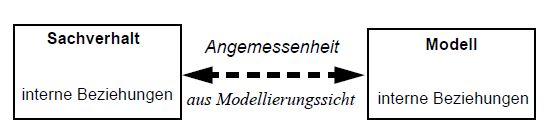
\includegraphics[width=\textwidth]{Graphics/Sachverhalt.jpg}
		\captionof{figure}{Beziehung zwischen Modell und zu modellierendem Sachverhalt, Quelle : \cite[35]{Frank_1997}}
		\label{fig:Beziehung}
	\end{figure}
Sollte ein Modell nicht formal definiert sein, so ist die einzige Möglichkeit, den Inhalt dessen zu erfassen und mit dem gegebenen Sachverhalt entgegen zu prüfen. Je nachdem wie exakt und präzise ein Modell interpretiert werden kann, desto leichter kann es mit dem abzubildenden Sachverhalt verglichen werden. Es ist zwar prinzipiell nicht zu entscheiden, ob ein unpräziser Sachverhalt und ein präzises Modell adäquat sind, jedoch hilft die Präzession und Genauigkeit eines Modells bei dem Vergleich des abzubildenden Sachverhalts. Eine Modellierungssprache, die es ermöglicht, Modelle exakt und eindeutig zu beschreiben
und zu interpretieren, erleichtert daher die Überprüfung des Modells wesentlich. Ist das Modell eindeutig, so ist auch ein umfängliches übergreifendes Verständnis möglich. Dies bedeutet aber auch, das jedes Sprachkonstrukt und Sprachverhalten eindeutig interpretiert werden muss. Ansonsten kann dies wegen Interpretationsschwierigkeiten zu Missverständnissen führen. Deswegen muss eine abstrakten Syntax und Semantik vorausgesetzt werden, um die Interpretation der Modelle zu vereinheitlichen \cite[35F]{Frank_1997}.


